\clearpage
\subsection{Statement} % (fold)
\label{sub:statement}

A statement is an instruction for the computer to perform an action, a command telling it what to do. Each \nameref{sub:program} contains a list of statements (commands). When the program is run the computer follows these commands one at a time, in sequence, starting at the program's entry point and ending when it completes the program's last statement.

\begin{figure}[h]
   \centering
   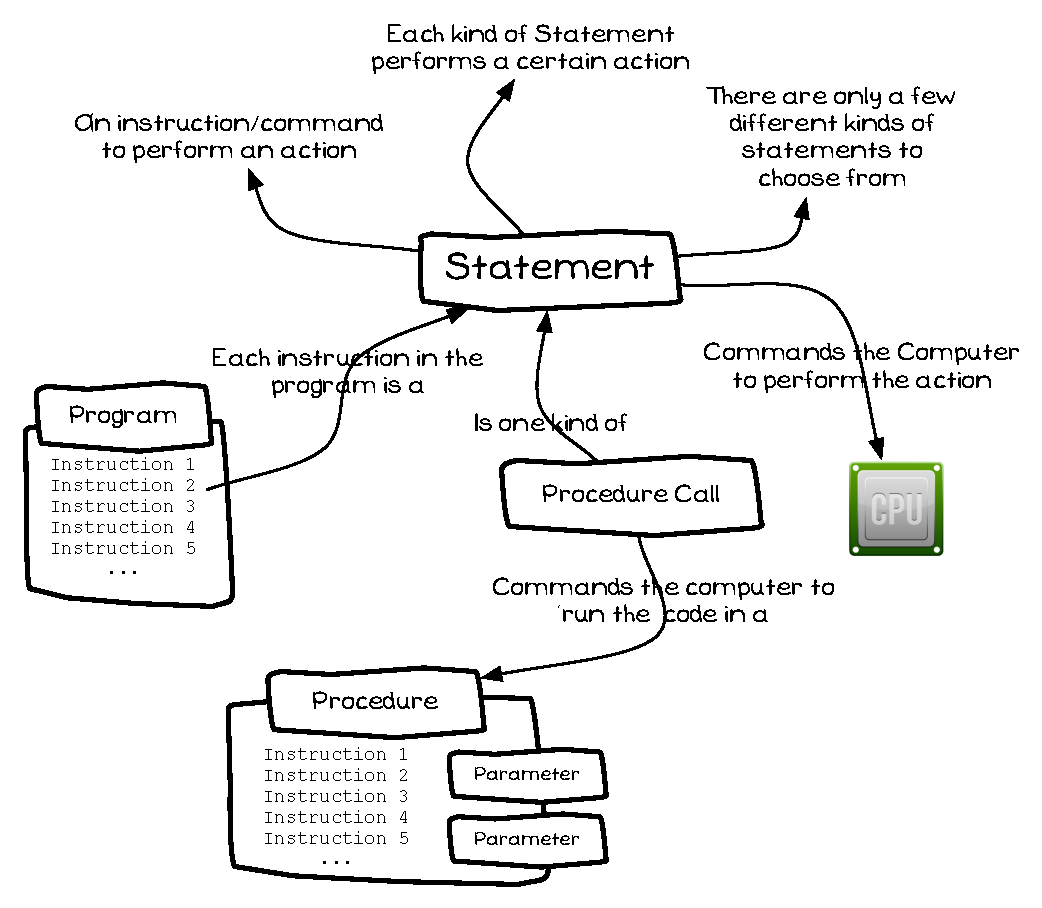
\includegraphics[width=\textwidth]{./topics/program-creation/diagrams/Statement} 
   \caption{A statement is a command for the computer to perform an action}
   \label{fig:program-creation-statement}
\end{figure}


\mynote{
\begin{itemize}
  \item A statement is a \textbf{term} used to describe the instructions in your code.
  \item Figure \ref{fig:program-creation-statement} shows the concepts related to statements.
  \item A statement is a \textbf{command}, an instruction to perform a task.
  \item A \nameref{sub:program} has a list of statements that are followed when it is executed.
  \item There are only a few different kinds of statement.
  \item A \nameref{sub:procedure call} is a kind of statement, it tells the computer to run the code in a \nameref{sub:procedure}.
  \item This style of programming is known as \textbf{Imperative} programming. Imperative means to give authoritative commands, and that is what we do in our programs. Our programs are lists of authoritative commands telling the computer to perform actions.
\end{itemize}
}

% section statement (end)